\begin{multicols*}{2}

    \chapter{Infraestructura física y puesta a punto}
    
    \section{Primer contacto con la infraestructura física}
    
    El comienzo de este proyecto arrancó con mi primer contacto real con el hardware: la puesta a punto del servidor Dell PowerEdge R7615 en las instalaciones del Centro de Transferencia Tecnológica de la UGR. Todo el proceso se realizó bajo la supervisión de los tutores del TFG, asegurando el cumplimiento de los protocolos de seguridad y las prácticas técnicas establecidas por el centro.
    
    \subsection*{Proceso de instalación}
    
    Antes de nada, como protocolo, se formalizó una solicitud de acceso detallando objetivos y requisitos técnicos, ya que el centro mantiene un control exhaustivo de quién entra y de quién sale, dado que la sala de servidores es un punto crítico de información y servicio para la universidad.
    
    \begin{center}
        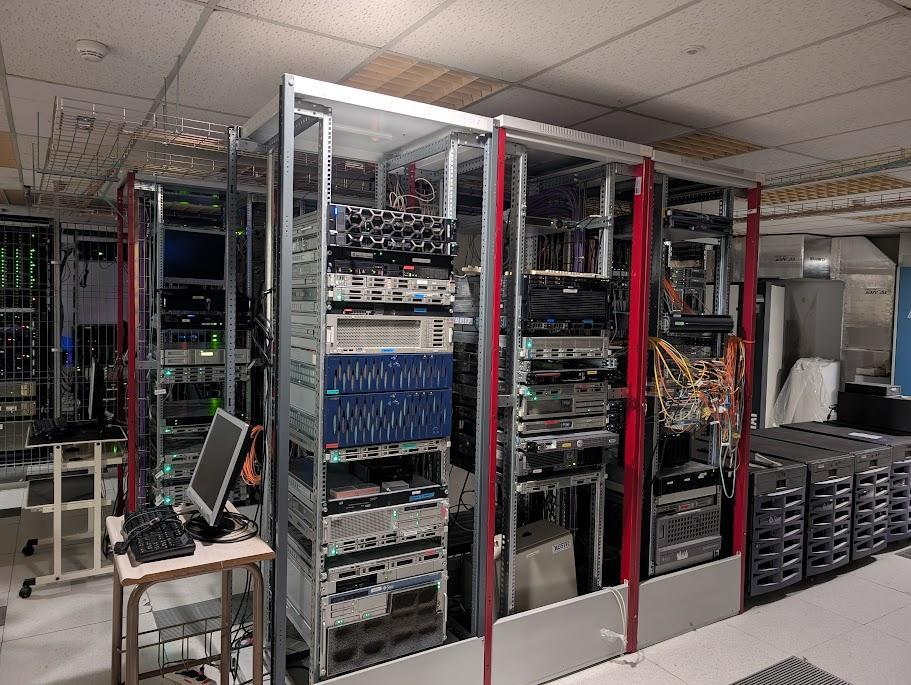
\includegraphics[width=0.95\linewidth]{imagenes/image12.jpg}
        \captionof{figure}{Server Room del CTT de la UGR}
        \label{fig:server-room}
    \end{center}
    
    El montaje se llevó a cabo en un rack estándar de 42U, respetando las distancias mínimas de ventilación (aprox. $\geq$30 cm por delante y por detrás) para evitar el sobrecalentamiento. Las instalaciones cuentan con control de temperatura para proteger los servidores.
    
    \begin{center}
        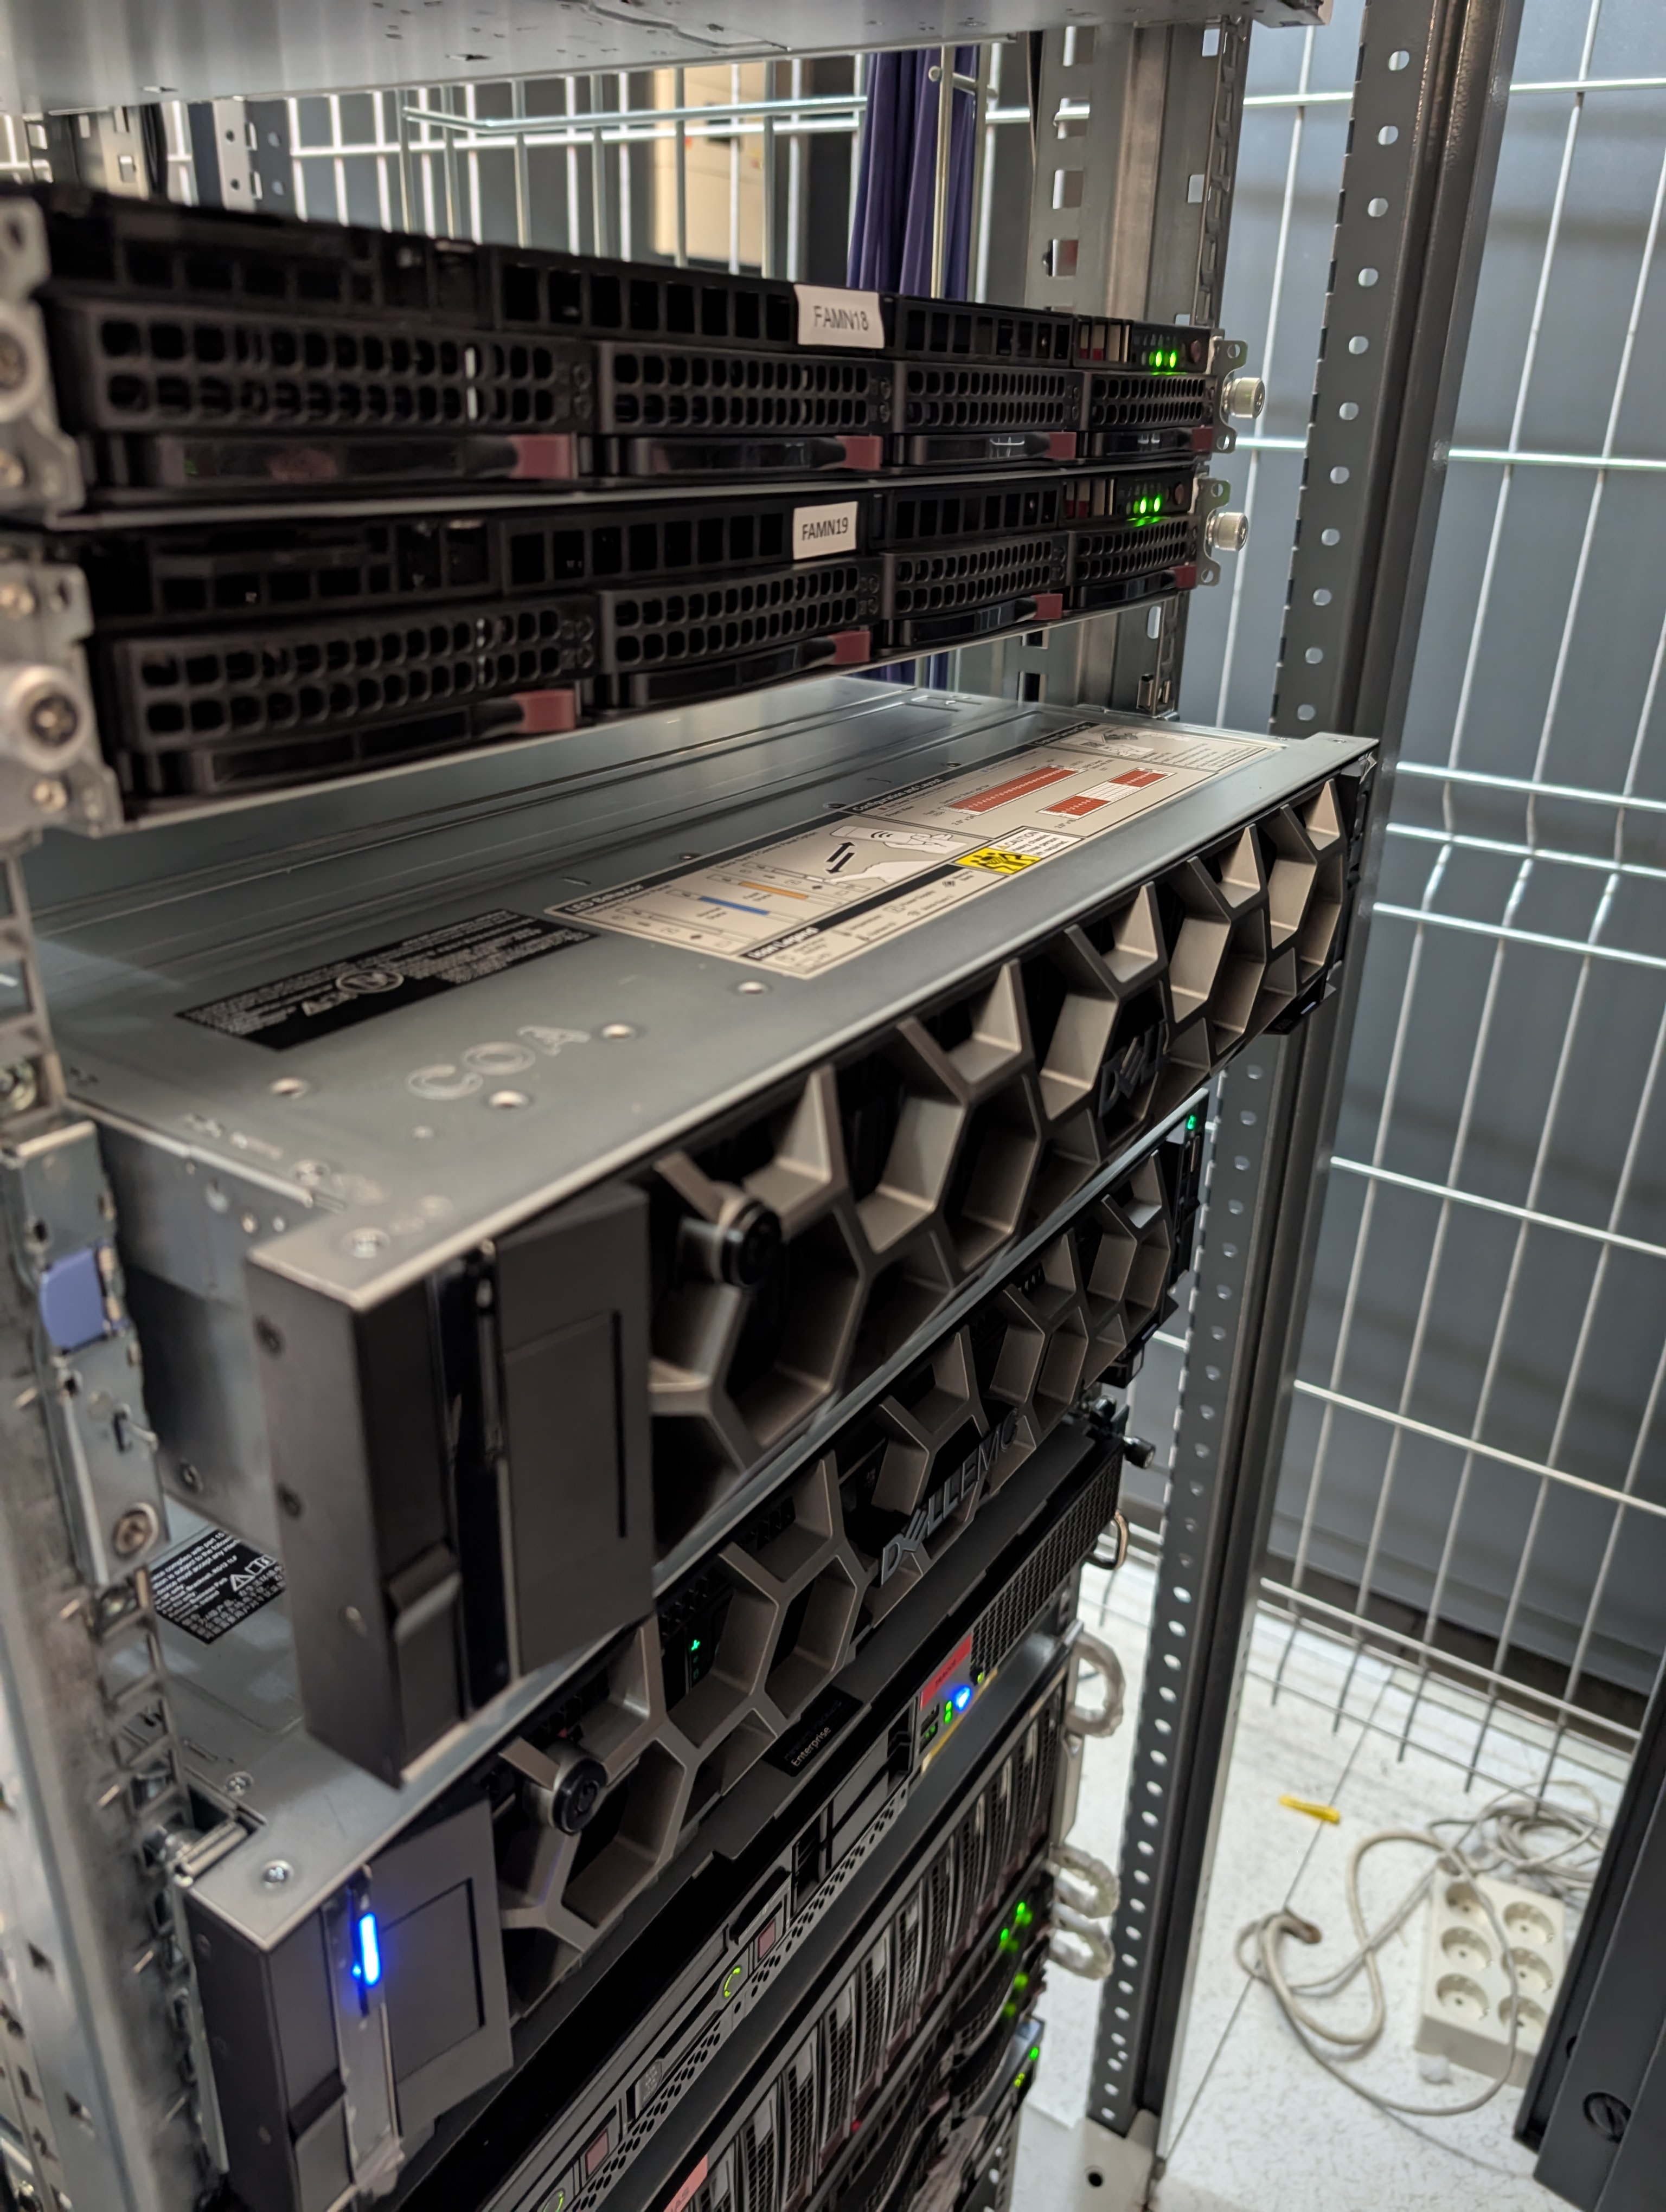
\includegraphics[width=0.85\linewidth]{imagenes/PXL_20250113_100402730.jpg}
        \captionof{figure}{Montaje del servidor Dell PowerEdge R7615}
        \label{fig:montaje-servidor}
    \end{center}
    
    Se instalaron dos fuentes de alimentación separadas y conexiones de red de alta velocidad a 10Gbps, asegurando redundancia y continuidad ante posibles fallos.
    
    Durante la instalación, un pequeño accidente me hizo reflexionar sobre la importancia de los detalles: al desempaquetar el servidor, me corté con el borde de la caja. Mi tutor reaccionó rápidamente con el botiquín, recordándome que, más allá de la tecnología, los pequeños imprevistos pueden afectar el desarrollo de un proyecto.
    
    \begin{center}
        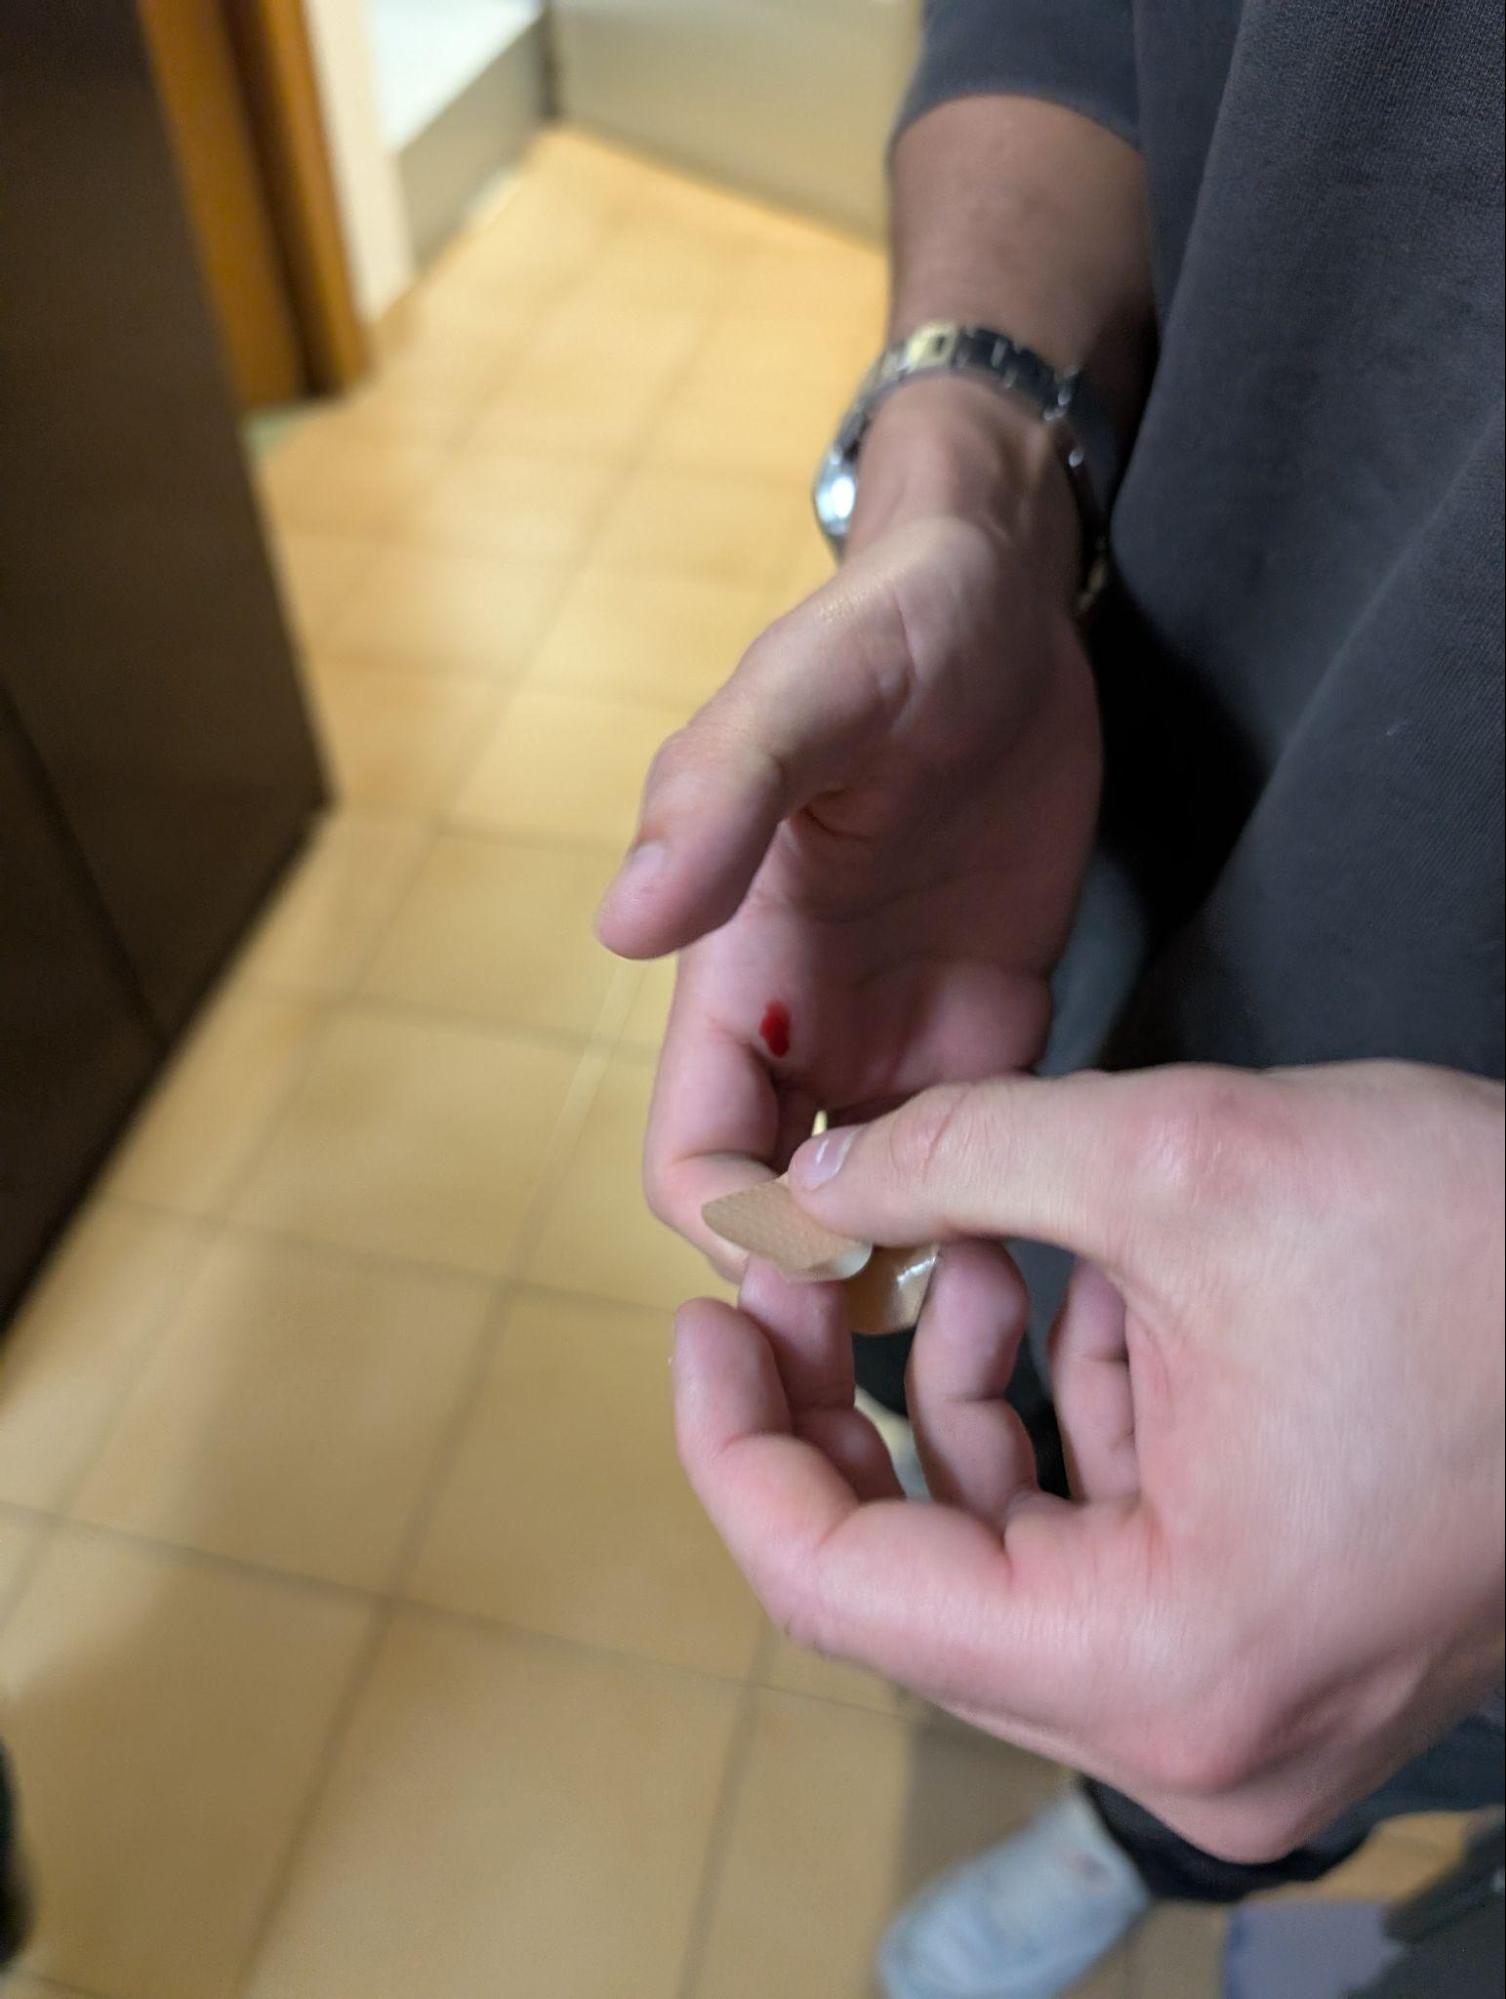
\includegraphics[width=0.95\linewidth]{imagenes/image16.jpg}
        \captionof{figure}{Detalle durante la instalación}
        \label{fig:detalle-instalacion}
    \end{center}
    
    Esta experiencia refuerza la filosofía de Site Reliability Engineering: tan importante es la arquitectura como la capacidad de anticipar y resolver pequeños problemas cotidianos.
    
    \subsection*{Experiencia Práctica y Consideraciones sobre la Instalación}
    
    Cabe señalar que, para el servidor específico de este proyecto, la instalación del sistema operativo y el cableado fueron gestionados por el personal técnico del centro universitario. Sin embargo, este aspecto fue complementado por la experiencia adquirida en mis prácticas Erasmus en la empresa Desion, en Darmstadt, Alemania.
    
    Durante estas prácticas como IT Infrastructure, me responsabilicé del setup de servidores para aplicaciones de IA, incluyendo el montaje físico de componentes como CPU y GPU, y el cableado entre otros. Adicionalmente, di soporte a la automatización de infraestructura, monitoricé el rendimiento y la disponibilidad de sistemas, optimicé pipelines CI/CD y aprendí la importancia de la documentación técnica durante las instalaciones. Para estas tareas, utilicé herramientas como Nagios y Grafana, y perfeccioné mi uso de Docker para el despliegue de servicios empresariales, como la herramienta de anotación de datos CVAT con Traefik.
    
    Un ejemplo clave fue la instalación completa de Ubuntu 22.04 LTS en dos servidores Supermicro. Esta tarea me permitió comprender la importancia de las versiones LTS (Long Term Support), que garantizan actualizaciones de seguridad y estabilidad a largo plazo, frente a versiones más recientes que pueden presentar incompatibilidades. Esta experiencia fue importante para mi desarrollo profesional, ofreciéndome una perspectiva práctica sobre el ciclo de vida del software y las decisiones estratégicas en la selección del sistema operativo, así como una base sólida en el despliegue y mantenimiento de infraestructuras.
    
    \begin{center}
        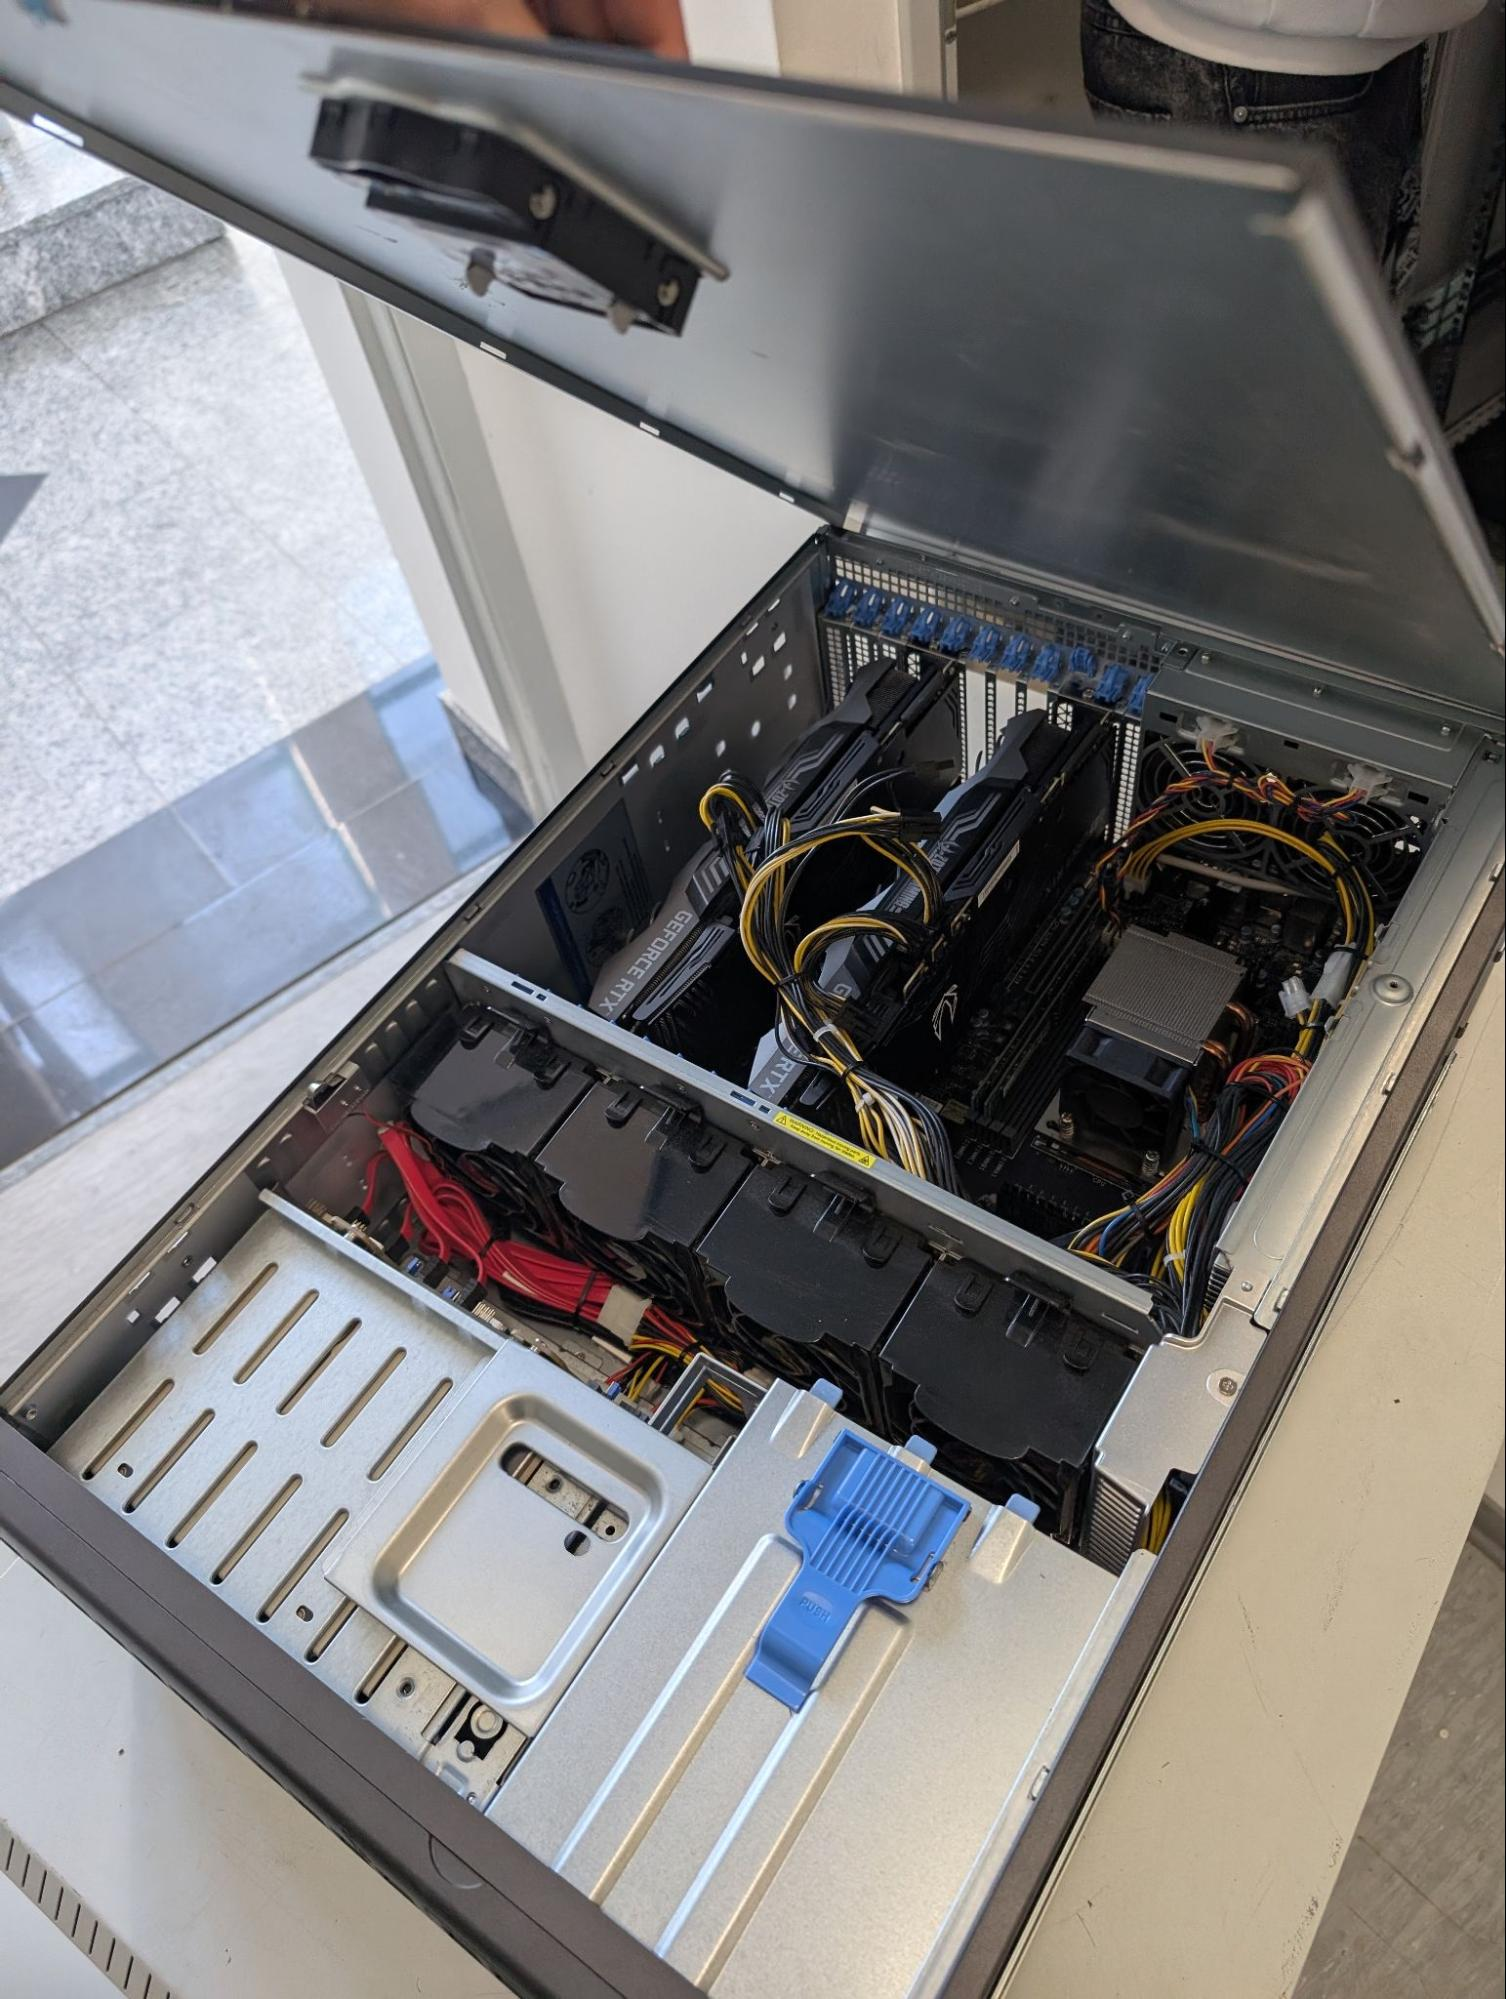
\includegraphics[width=0.95\linewidth]{imagenes/image4.jpg}
        \captionof{figure}{}
        \label{fig:detalle-instalacion2}
    \end{center}

    % cableado + sre

    Otro ejemplo relevante de puesta a punto de infraestructura ocurrió durante mi viaje a Schwechat (Austria), donde realicé la instalación física de los servidores mostrados en la imagen anterior. En esta ocasión, no solo participé en el montaje físico de los equipos en un rack estándar de 42U, sino también en la planificación y ejecución del cableado estructurado, tanto de red como de alimentación. El armario se instaló, y se instalaron los siguientes componentes: un panel de distribución de fibra óptica, dos servidores Dell PowerEdge equipados cada uno con una CPU AMD EPYC y cuatro GPUs NVIDIA L4, un servidor Fujitsu, un SAI APC (Sistema de Alimentación Ininterrumpida) y un switch de red de alto rendimiento con conectividad de 10 Gbps. Todos los equipos se organizaron con gestores de cableado para facilitar el mantenimiento y asegurar una buena ventilación. En cuanto al sistema operativo, instalé Ubuntu 22.04 LTS en ambos servidores Dell y el Futjitsu. 

    Para asegurar la monitorización del sistema, se configuró Nagios en el servidor Fujitsu. Este servidor actuó como nodo de control, vigilando el estado de los otros dos mediante chequeos periódicos de disponibilidad, uso de recursos y estado de red. Esta capacidad de monitorización es clave para anticipar fallos y garantizar la disponibilidad, un principio fundamental del enfoque SRE.

    \begin{center}
        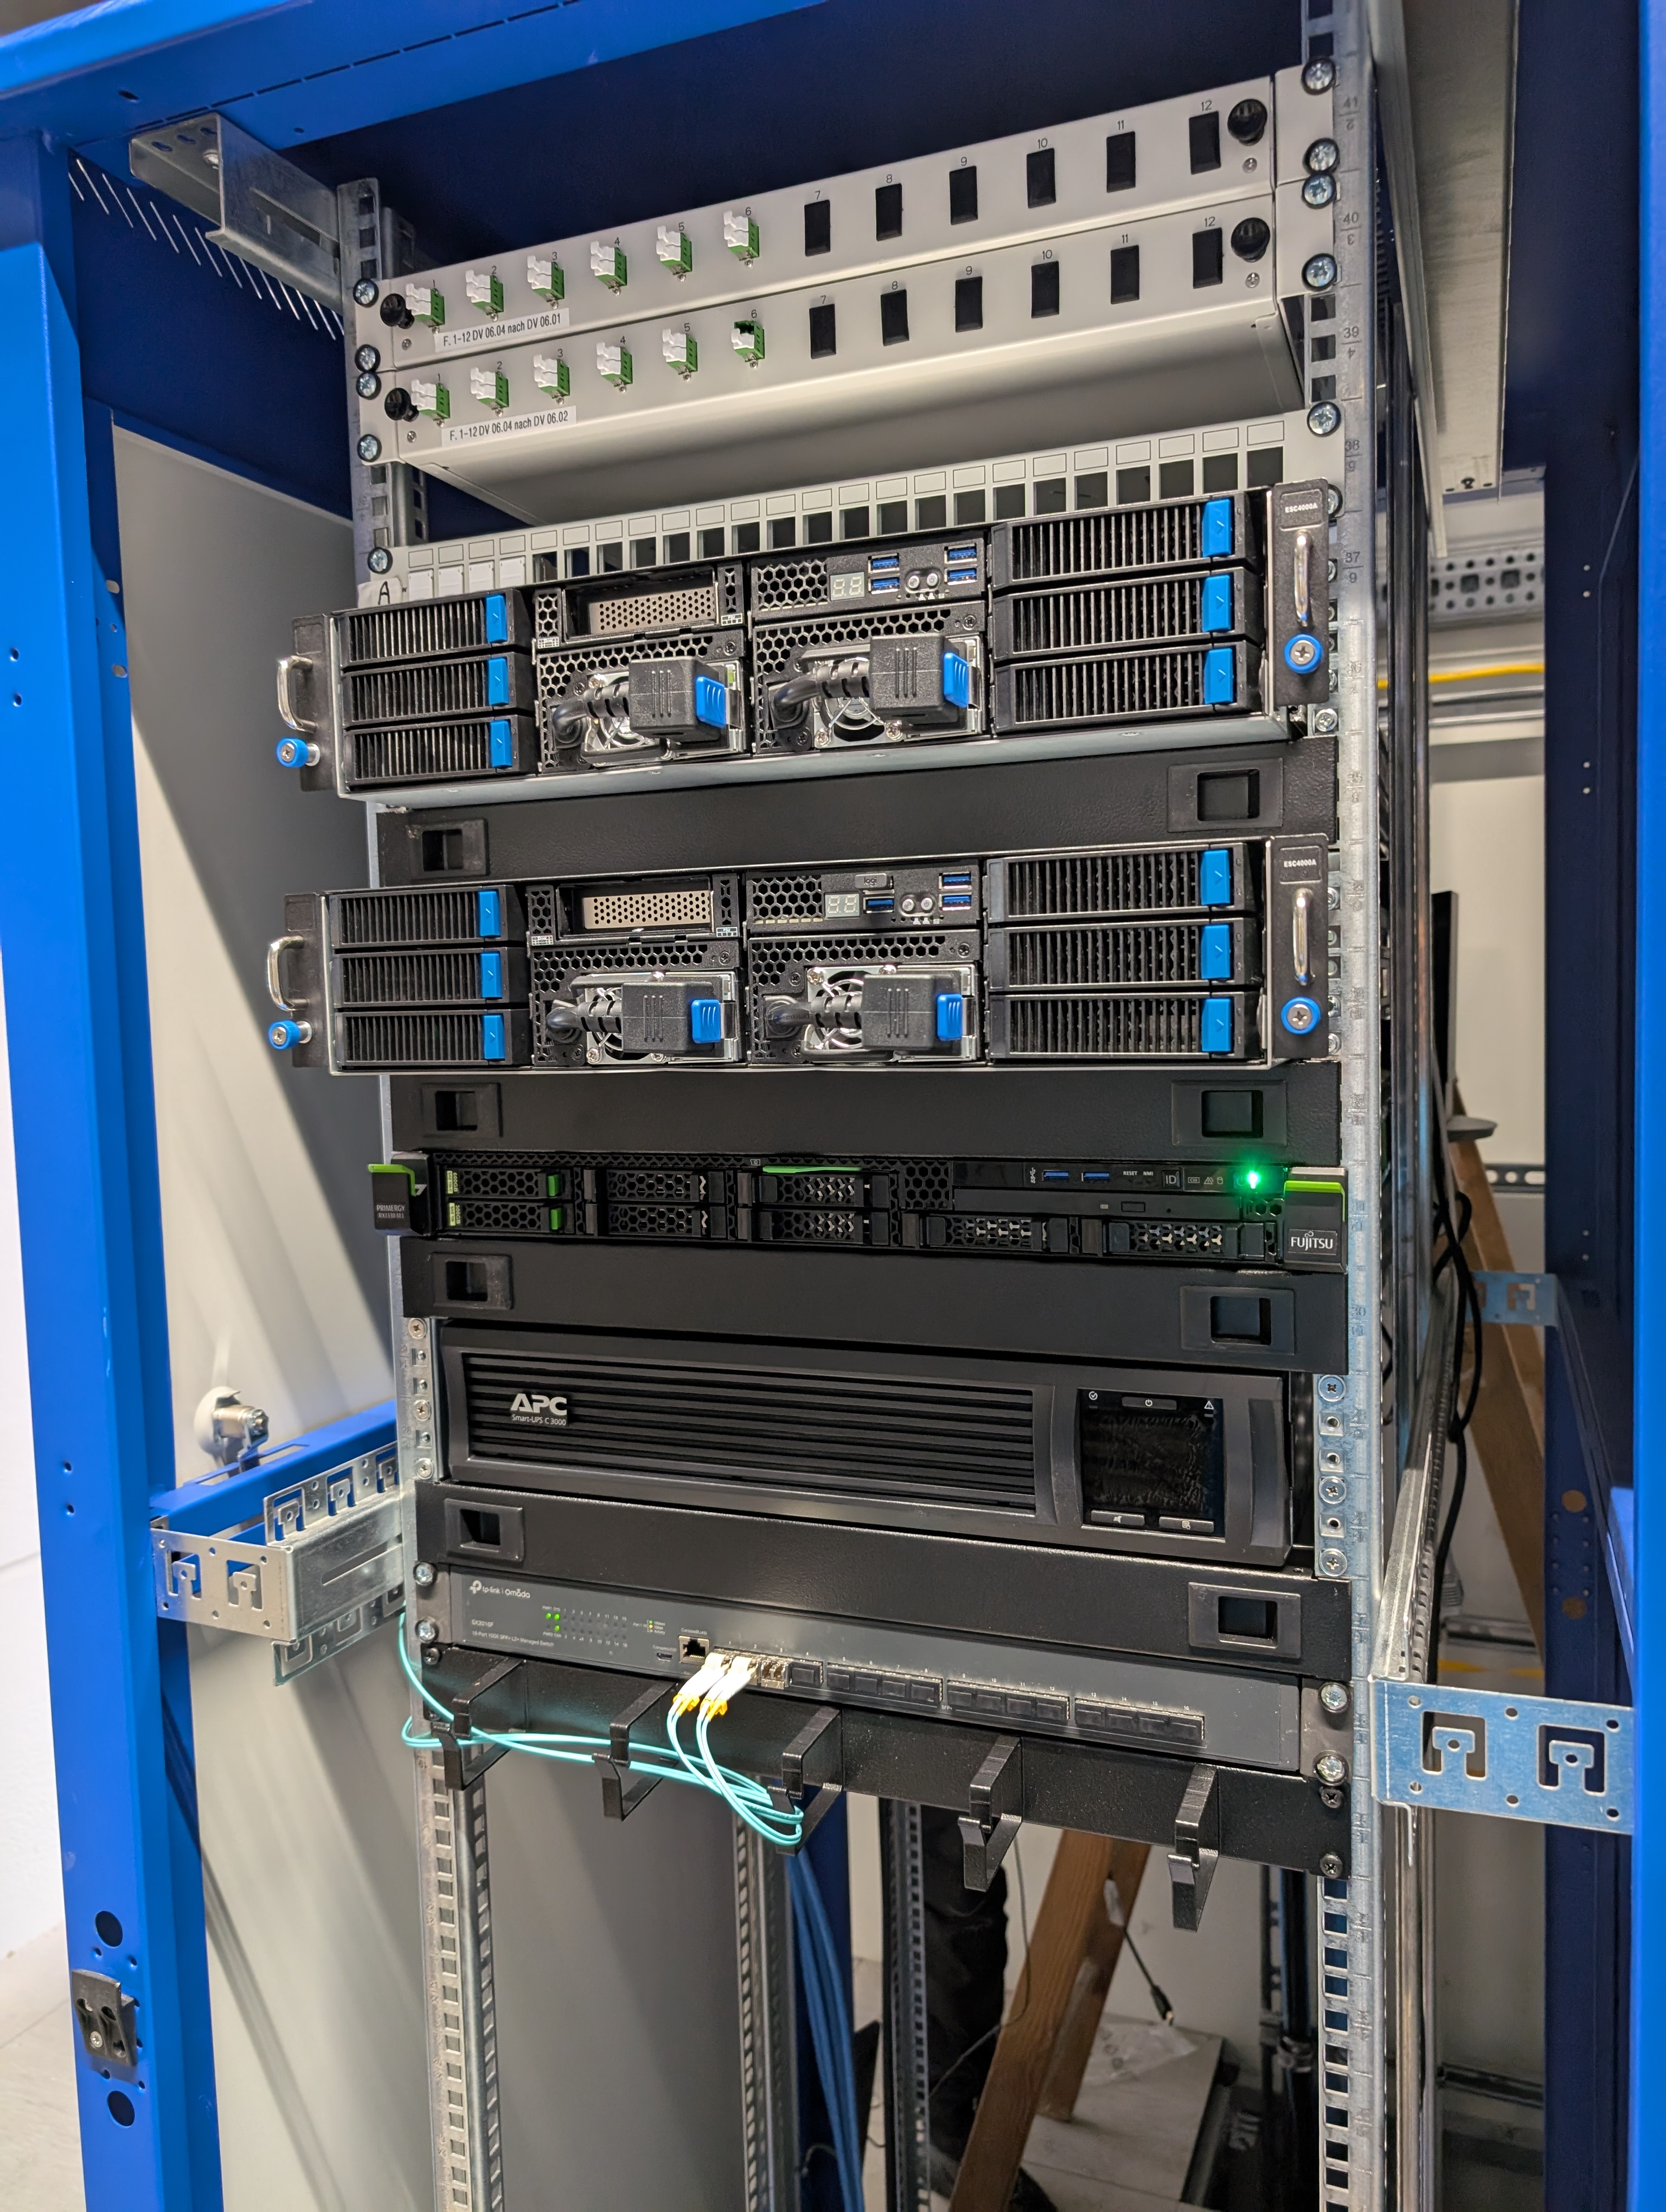
\includegraphics[width=0.95\linewidth]{imagenes/PXL_20250513_075406997.jpg}
        \captionof{figure}{}
        \label{fig:detalle-instalacion2}
    \end{center}

    \newpage
    \section{Conexión Remota y Acceso al Servidor}

    La operación del servidor, ubicado en la Universidad de Granada (España), se realiza de forma remota desde Darmstadt (Alemania), donde se llevan a cabo las prácticas extracurriculares en la empresa Desion. Esto exige una conexión remota eficiente para el desarrollo del TFG.

    Es crucial reconocer que el acceso remoto es un punto crítico de seguridad en cualquier infraestructura. Por ello, siempre se recomienda aplicar principios como la restricción de privilegios, la trazabilidad mediante auditorías y la automatización dentro de lo posible. Esto minimiza errores humanos y aumenta la resiliencia operativa.

Para el acceso se emplea SSH (Secure Shell), un protocolo estándar que cifra la comunicación en red. Aunque el puerto por defecto de SSH es el 22, su uso predeterminado lo convierte en un objetivo frecuente de ataques automatizados, como los de fuerza bruta. Utilizar puertos no estándar, como el usado en el servidor principal, en este caso, reduce la exposición directa a estos escaneos y aumenta la seguridad.

Aunque se intentó una conexión directa vía VPN, problemas de configuración en el servidor principal impidieron esta opción. Por ello, se optó por una alternativa que requiere dos saltos de conexión: el primero a una máquina intermedia (máquina-A) y el segundo al servidor objetivo (máquina-B). Por motivos de seguridad, y para proteger información sensible, los nombres de host y usuarios específicos se omiten en esta documentación. La metodología de conexión se detalla a continuación.

\subsubsection*{Pasos para la Conexión Remota}

\noindent\textbf{1. Conexión a la Máquina Intermediaria (Máquina A)}\\
La conexión se establece primero con una máquina intermedia de la Universidad de Granada. Este paso es necesario debido a la imposibilidad de una conexión VPN directa con el servidor principal.

\begin{center}
\begin{minipage}{0.95\linewidth}
\begin{verbatim}
ssh user@maquina-a
\end{verbatim}
\end{minipage}
\end{center}


\noindent\textbf{2. Conexión a la Máquina de Trabajo (Máquina B)}\\
Desde la máquina intermedia, se accede al servidor HPC. Se utiliza el mismo usuario que en el paso anterior. En este caso se ha abierto un puerto en específico para entrar al servidor.

\begin{center}
\begin{minipage}{0.95\linewidth}
\begin{verbatim}
ssh maquina-b -p XXXXX -vvv
\end{verbatim}
\end{minipage}
\end{center}

\noindent\textbf{Puerto -p:} Se especifica un puerto no estándar por motivos de seguridad..\\
\textbf{Opciones -vvv:} \texttt{-vvv} La opción -vvv muestra información detallada de la conexión, lo cual fue crucial para depurar problemas. Se utilizó principalmente al intentar conectar directamente con la VPN de la universidad activa, lo que permitió identificar que la VPN no estaba realizando el tunneling correctamente porque el servidor no estaba configurado para ello.

\subsubsection*{Configuración de Autenticación por Clave SSH}

Para simplificar y asegurar el acceso, se automatiza el proceso mediante autenticación por clave SSH en lugar de contraseñas, lo que evita la necesidad de introducir credenciales múltiples veces. Este método se aprendió y aplicó durante las prácticas en Alemania. La autenticación por clave mejora significativamente la seguridad al eliminar el riesgo de ataques de fuerza bruta basados en contraseñas y la exposición de credenciales, además de automatizar el acceso. Este procedimiento se realiza con la autorización del tutor.

\vspace{\baselineskip}

\noindent\textbf{1. Generar una Clave SSH}

Se genera un par de claves SSH en la máquina local. Se recomienda el algoritmo ed25519 por su seguridad y eficiencia. Ed25519 es un algoritmo de criptografía de curva elíptica relativamente moderno que se ha vuelto muy recomendado y cada vez más utilizado para claves SSH. 

\begin{center}
\begin{minipage}{0.95\linewidth}
\begin{verbatim}
ssh-keygen -t ed25519 \
-C "correo-usuario"
\end{verbatim}
\end{minipage}
\end{center}

\noindent \textbf{Tipo de Clave:} \texttt{ed25519} (algoritmo moderno y seguro).\\
\textbf{Comentario:} Se utiliza un correo electrónico para identificar la clave.\\
Passphrase: Puede dejarse vacía si no se requiere una capa adicional de seguridad.\\

\noindent La clave pública se guarda en \texttt{\~{}/.ssh/id\_ed25519.pub} y la privada en \texttt{\~{}/.ssh/id\_ed25519}.

\vspace{\baselineskip}

\noindent\textbf{2. Copiar la Clave Pública a la Máquina A}

La clave pública se copia a la máquina intermedia para establecer la confianza. Se emplea ssh-copy-id para una transferencia rápida y segura.

\begin{center}
\begin{minipage}{0.95\linewidth}
\begin{verbatim}
ssh-copy-id user@maquina-a
\end{verbatim}
\end{minipage}
\end{center}

\columnbreak

\noindent\textbf{3. Copiar la clave Pública a la Máquina B}

A continuación, la misma clave pública se copia al servidor HPC (máquina B).

\begin{center}
\begin{minipage}{0.95\linewidth}
\small
\begin{verbatim}
echo "ssh-ed25519 mi-clave" | \
ssh -p XXXX user@maquina-b "\
mkdir -p ~/.ssh; \
cat >> ~/.ssh/authorized_keys; \
chmod 700 ~/.ssh; \
chmod 600 ~/.ssh/authorized_keys"
\end{verbatim}
\end{minipage}
\end{center}

\noindent Contenido de la Clave: Se debe reemplazar \textbf{\texttt{[contenido\_de\_tu\_clave\_publica]}} con el texto exacto de tu archivo \texttt{\~{}/.ssh/id\_ed25519.pub}.\\
\textbf{Permisos:} El comando asegura que los directorios y archivos tengan los permisos adecuados para la seguridad de SSH.

\vspace{\baselineskip}

\noindent\textbf{4. Verificación de la Conexión}

\begin{center}
\begin{minipage}{0.95\linewidth}
\begin{verbatim}
ssh -J user@maquina-a \ 
user@maquina-b -p XXXX
\end{verbatim}
\end{minipage}
\end{center}
\textbf{Opción } \textbf{-J}: Usa la máquina A como salto intermedio para llegar a la máquina B.

\vspace{\baselineskip}

\noindent\textbf{5. Configuración del Archivo ~/.ssh/config}

Para simplificar la conexión y evitar comandos largos, se edita el archivo de configuración SSH en la máquina local (~/.ssh/config) añadiendo las siguientes entradas:

\begin{center}
\begin{minipage}{0.95\linewidth}
\begin{verbatim}
Host maquina-a
    HostName maquina-a
    User user

Host maquina-b
    HostName maquina-b
    User user
    Port XXXXX
    ProxyJump maquina-a
\end{verbatim}
\end{minipage}
\end{center}



\end{multicols*}

\begin{minipage}[t]{0.48\textwidth} 
    Con todo esto hemos logrado conectarnos a nuestro servidor con simplemente este comando:

    \begin{center}
    \begin{minipage}{0.95\linewidth}
    \begin{verbatim}
$ ssh maquina-b
    \end{verbatim}
    \end{minipage}
    \end{center}
    
    \begin{center}
       \begin{minipage}{0.95\linewidth}
       \small
       \begin{verbatim}
1 dispositivo tiene una \
actualización disponible.
Ejecute `fwupdmgr get-upgrades` \
para más información.
       
Last login: Fri Apr  4 16:43:37 \
2025 from X.X.X.X
[user@maquina-b ~]$
       \end{verbatim}
       \end{minipage}
       \end{center}
    
    Este proceso de autenticación basada en claves y configuración optimizada minimiza la intervención manual y reduce la complejidad del acceso, permitiendo centrar los esfuerzos en las tareas del proyecto.
    
    \section{Especificaciones del servidor}
    
    Tras conocer cómo conectarnos al servidor, damos paso a estudiar la infraestructura con la que trabajo, qué componentes la forman. 
    

\end{minipage}%
\hfill 
\begin{minipage}[t]{0.46\textwidth} 
    
    Instalando \texttt{neofetch} podemos ver sus especificaciones de manera sencilla, vamos a analizarla.
    
    \subsubsection*{Sistema Operativo}
    El servidor utiliza Fedora Linux 41 en su edición para servidores,    una distribución robusta y actualizada diseñada para entornos empresariales ofreciendo robustez y estabilidad. Tiene una arquitectura de \texttt{x86\_64}, compatible con procesadores de 64 bits y un rendimiento óptimo en tareas que requieren gran capacidad de cómputo. El kernel que usa es la versión \texttt{6.13.8-200.fc41.x86\_64}, reciente y con mejoras en seguridad, soporte de hardware y optimizaciones de rendimiento.

    \subsubsection*{Procesador (CPU)}
    El procesador instalado es un AMD EPYC 9334, basado en la arquitectura Zen 4 de la serie EPYC 9004. Este modelo destaca por su eficiencia energética y capacidad para procesamiento paralelo, características ideales para servidores. 

\end{minipage}

\begin{figure}[H]
    \centering
    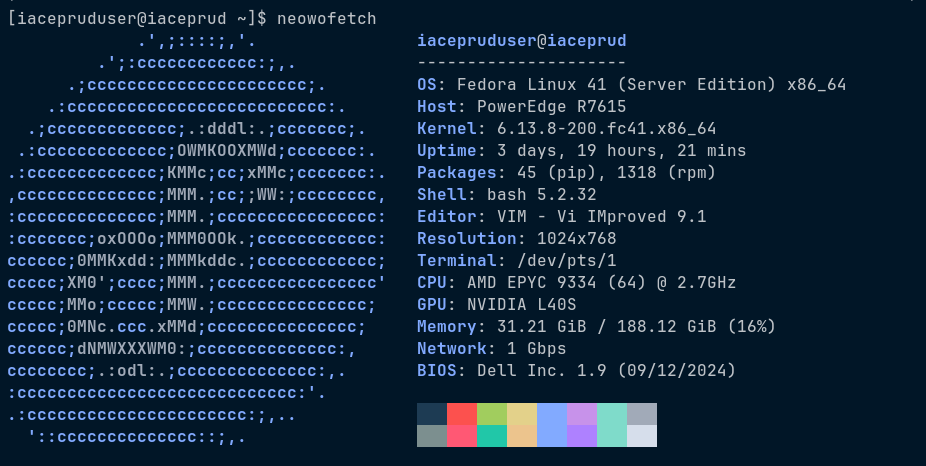
\includegraphics[width=0.8\linewidth]{imagenes/image19.png}
    \caption{Comparison of Kubernetes, Docker Swarm, Mesos and OpenShift}
    \label{fig:server2}
\end{figure}

\newpage

\begin{multicols*}{2}

Aunque el EPYC 9334 tiene 32 núcleos y 64 hilos por socket, el sistema reporta 64 núcleos físicos, lo que sugiere la presencia de dos sockets, lo que elevaría la capacidad total a 64 núcleos y probablemente 128 hilos. Esto lo convierte en una unidad excepcionalmente potente para tareas multinúcleo. Su frecuencia base es de 2.7 GHz, con capacidad para aumentar mediante turbo bajo demanda, optimizando el rendimiento en momentos de alta carga.

\subsubsection*{Memoria RAM}
Tiene 188.12 GiB de memoria RAM, utilizando tecnología DDR5 con corrección de errores (ECC), un estándar en servidores que asegura la integridad de los datos y soporta aplicaciones intensivas en memoria. Actualmente, solo el 16\% de esta capacidad está en uso, equivalente a 31.21 GiB, lo que deja un amplio margen para manejar cargas adicionales sin comprometer el rendimiento, indicando una configuración bien adaptada a las tareas actuales.


\subsubsection*{Unidad de Procesamiento Gráfico (GPU)}
El servidor está equipado con una NVIDIA L40S, una GPU de alto rendimiento diseñada para tareas avanzadas como inteligencia artificial, aprendizaje profundo, renderizado y computación científica. Esta unidad complementa la capacidad del servidor al ofrecer potencia adicional para procesamiento paralelo y aplicaciones que requieren cálculos gráficos intensivos, lo que la hace ideal para entornos que demandan un alto nivel de cómputo más allá de las capacidades de la CPU.

\subsubsection*{Red}
\begin{verbatim}
$ lspci | grep -i ethernet
\end{verbatim}

El sistema cuenta con múltiples interfaces de red Broadcom NetXtreme, incluyendo dos controladoras 10G RDMA Ethernet. Estas proporcionan alta velocidad de transmisión y baja latencia, aspectos fundamentales para mantener la disponibilidad y la fiabilidad del sistema.

Desde la perspectiva del Site Reliability Engineering, conocer en detalle estas especificaciones no es solo una cuestión informativa, sino una parte integral de la construcción de sistemas resilientes. Tal como se recomienda en las buenas prácticas de SRE, disponer de visibilidad clara sobre la infraestructura permite anticipar cuellos de botella, planificar escalabilidad y establecer mecanismos de recuperación más eficaces.

\subsection*{¿Es la infraestructura un HPC?}

La infraestructura analizada cumple con varios requisitos clave de un sistema de computación de alto rendimiento (HPC). El servidor Dell PowerEdge R7615, con Fedora Linux 41, proporciona una base robusta para cargas intensivas. Su procesador AMD EPYC 9334, con 64 núcleos y 128 hilos, junto con la GPU NVIDIA L40S orientada a IA, permite un alto paralelismo y cómputo acelerado. La RAM de 188 GiB DDR5 con ECC asegura un manejo eficiente de grandes volúmenes de datos. Aunque dispone de interfaces de red de hasta 10 Gbps, actualmente opera con una conexión de 1 Gbps, suficiente para un nodo aislado, pero limitada para un entorno HPC distribuido.

Por tanto, aunque el hardware es claramente HPC, su clasificación como sistema HPC depende del contexto operativo, no se trata de un clúster distribuido con múltiples nodos ni de una arquitectura gestionada mediante herramientas como MPI o SLURM. En su estado actual, puede considerarse un nodo de alto rendimiento preparado para tareas intensivas, pero no un sistema HPC completo.

No obstante, el uso de herramientas de orquestación como OpenShift permite desplegar servicios, simulando parcialmente el comportamiento y la gestión de cargas típico de un entorno HPC. A través de esta plataforma, es posible automatizar la asignación de recursos, escalar servicios y supervisar el rendimiento del sistema, características clave en arquitecturas distribuidas. Aunque la infraestructura se limite a un único servidor, la experiencia de operar en este entorno proporciona una aproximación práctica al modelo HPC.


\vspace{\baselineskip}

\section{Instalar los Drivers}

Se asignó la responsabilidad de instalar los controladores NVIDIA en el servidor, el cual es compartido con otros dos estudiantes. Aunque la instalación de drivers y entornos CUDA es una tarea habitual gracias a mi experiencia en prácticas, el sistema operativo actual, Fedora Linux 41, representa un contexto distinto que exige mayor precaución en comparación con distribuciones como Debian.

\vspace{\baselineskip}


\noindent\textbf{NVIDIA Optimus y su Relevancia:} 

Optimus es una tecnología de NVIDIA que integra una GPU dedicada con una GPU integrada para optimizar rendimiento y eficiencia energética. En este servidor, que incluye una GPU NVIDIA L40S junto a una GPU integrada (Matrox G200eW3), el enfoque principal es instalar los controladores que permitan aprovechar la GPU dedicada en un entorno sin interfaz gráfica.

\vspace{\baselineskip}

\noindent\textbf{Pasos para la instalación:}

\vspace{\baselineskip}

\noindent\textbf{1. Añadir los repositorios RPM Fusion}

Primero, se añaden los repositorios RPM Fusion, necesarios para obtener los paquetes de drivers no libres.

\begin{verbatim}
sudo dnf update
sudo dnf install \ 
\url{https://download1.rpmfusion.org
/free/fedora/rpmfusion-free-release-
$(rpm -E \%fedora).noarch.rpm} \url
{https://download1.rpmfusion.org/non
free/fedora/rpmfusion-nonfree-release
-$(rpm -E \%fedora).noarch.rpm}
\end{verbatim}


\noindent Se verifica:
\begin{verbatim}
sudo dnf repolist | grep \
-i rpmfusion
\end{verbatim}

\vspace{\baselineskip}

\noindent\textbf{2. Actualizar el sistema}
\begin{verbatim}
sudo dnf upgrade --refresh
\end{verbatim}

\vspace{\baselineskip}

\noindent\textbf{3. Ver qué paquetes vamos a instalar}

Ahora, en forma de tabla, detallo qué paquetes hay que instalar. Hay que tener en cuenta que es un servidor sin interfaz gráfica, por lo que podemos ahorrarnos paquetes que no vamos a usar.

\begin{itemize}
    \item \texttt{gcc}: Compilador para construir módulos
    \item \texttt{kernel-headers}: Necesario para compilar módulos del kernel
    \item \texttt{kernel-devel}: Dependencia de akmod-nvidia
    \item \texttt{akmod-nvidia}: Módulo principal de los controladores NVIDIA
    \item \texttt{xorg-x11-drv-nvidia-libs}: Librerías esenciales para CUDA
    \item \texttt{nvidia-driver}: controlador de Nvidia, para tener nvidia-smi
\end{itemize}

\vspace{\baselineskip}

\noindent\textbf{4. Comprobar el Secure Boot}

Secure Boot puede bloquear controladores no firmados, es recomendable desactivarlo.
\begin{verbatim}
mokutil --sb-state
SecureBoot disabled
\end{verbatim}

Si está desactivado, no habrá problemas; de lo contrario, consulta con el tutor o administrador para desactivarlo.
\vspace{\baselineskip}

\noindent\textbf{5. Instalación de los paquetes}
\begin{verbatim}
sudo dnf install gcc \
kernel-headers \
kernel-devel

sudo dnf install \
akmod-nvidia \
xorg-x11-drv-nvidia-libs \
nvidia-drivers
\end{verbatim}

\vspace{\baselineskip}

\noindent\textbf{6. Construcción e instalación de los módulos}
\begin{verbatim}
sudo akmods --force
sudo dracut --force
sudo reboot
\end{verbatim}

\vspace{\baselineskip}

\noindent\textbf{7. Verificación con nvidia-smi}
    
Con esto vemos que hemos instalado Nvidia Drivers 570, compatibles con la gráfica y CUDA 12.8.

\vspace{\baselineskip}

\noindent\textbf{8. Instalar Cuda Toolkit}
    
Siguiendo las instrucciones oficiales de NVIDIA para Fedora 41 descargamos el paquete de repositorio de CUDA y lo añadimos al sistema. Esto nos permitirá instalar el toolkit de CUDA, que es esencial para desarrollar aplicaciones que aprovechen la GPU.:

\begin{verbatim}
$ sudo dnf config-manager addrepo\
--from-repofile \
https://developer.download.\
nvidia.com/compute/cuda/repos\
/fedora41/x86_64/cuda-fedora41.repo

$ sudo dnf clean all
    
$ sudo dnf -y install\
 cuda-toolkit-12-8
\end{verbatim}

\noindent\textbf{9. Configurar las variables de entorno}
\begin{verbatim}
$ echo 'export PATH=/usr/local/\
cuda/bin:$PATH' >> ~/.bashrc
echo 'export LD_LIBRARY_PATH=\
/usr/local/cuda/lib64:\
$LD_LIBRARY_PATH' >> ~/.bashrc

$ source ~/.bashrc
\end{verbatim}
\vspace{\baselineskip}

\noindent\textbf{10. Verificación de la instalación}
\begin{verbatim}
$ nvcc --version
... 
Build cuda_12.8.r12.8/compiler.35583870_0
\end{verbatim}

%nvcc: NVIDIA (R) Cuda compiler driver
%Copyright (c) 2005-2025 NVIDIA Corporation
%Built on Fri_Feb_21_20:23:50_PST_2025
%Cuda compilation tools, release 12.8, V12.8.93
%Build cuda_12.8.r12.8/compiler.35583870_0

Desde la perspectiva de los principios SRE, este tipo de tarea representa mucho más que una simple instalación técnica, se trata de operar infraestructura con responsabilidad, bajo el principio de que fiabilidad y seguridad van de la mano. Con todo esto se demuestra que las acciones de personas con acceso privilegiado deben ser predecibles, auditables y reproducibles, lo cual aplica incluso en tareas aparentemente rutinarias como esta.

Ya con todo esto, tenemos un servidor con las cualidades básicas, y podemos comenzar a desplegar LLM y servicios con OpenShift.

\vspace{\baselineskip}

\section*{Problemas Encontrados}

Tras completar la instalación de los controladores NVIDIA y reiniciar el sistema con \texttt{sudo reboot}, el servidor no volvió a estar disponible. Aunque intenté depurar el fallo mediante \texttt{ssh -vvv}, no logré identificar el problema, y fue necesaria intervención directa para recuperar la conexión con el servidor. Este incidente mostró cómo incluso acciones rutinarias como un reboot pueden generar fallos críticos si no se ejecutan con las precauciones adecuadas.

También evidenció una debilidad común en entornos reales: la falta de mecanismos de visibilidad y trazabilidad inmediata ante un fallo. No contar con registros accesibles, métricas previas al apagado o algún tipo de diagnóstico automatizado complica la identificación del origen del error y ralentiza la recuperación. Esto subraya la importancia de contar con buenas prácticas de observabilidad y de preparar el entorno para análisis post-fallo.

También, durante las prácticas, un problema similar ocurrió cuando un compañero realizó una actualización en el sistema, mientras que dicho servidor tenía Secure Boot activado. Esta función de seguridad del firmware UEFI verifica que el software cargado al arrancar, como el sistema operativo y los controladores, esté firmado digitalmente por un proveedor de confianza. En este caso, al instalarse controladores no firmados, Secure Boot bloqueó el arranque, dejando el sistema inutilizable. Gracias a que el rack estaba en nuestra oficina, pude resolverlo físicamente, pero esta situación demuestra cómo una configuración mal gestionada puede dejar fuera de servicio una máquina crítica, especialmente si no se tiene acceso físico inmediato o no se ha previsto un procedimiento de recuperación.

Estos eventos refuerzan la importancia de planificar operaciones sensibles como reinicios o actualizaciones: documentarlas, validarlas en entornos previos, y prever escenarios de recuperación. En ingeniería de fiabilidad, pequeños errores operativos pueden comprometer la disponibilidad de todo el sistema, y por eso deben tratarse con el mismo rigor que los fallos de software o hardware.

\end{multicols*}

\begin{figure}[H]
    \centering
    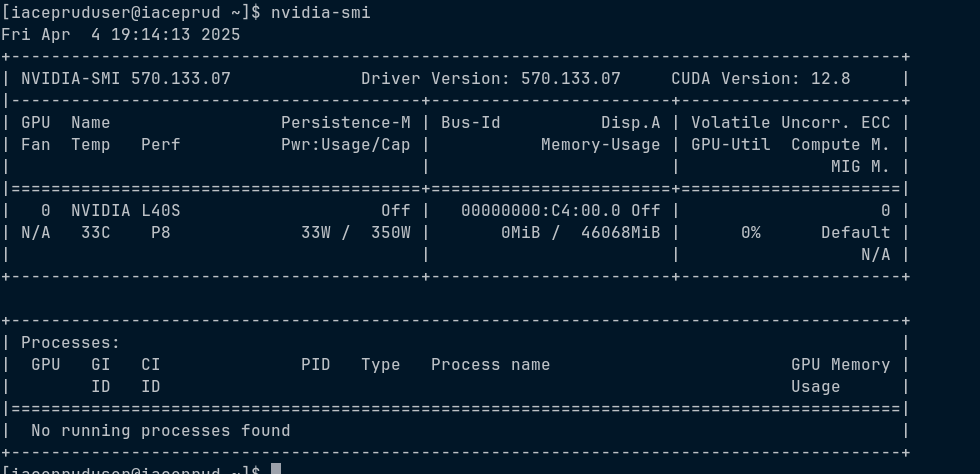
\includegraphics[width=\linewidth]{imagenes/image17.png}
    \caption{Comparison of Kubernetes, Docker Swarm, Mesos and OpenShift}
    \label{fig:server2}
\end{figure}

\newpage